\section{Algorithm: Geodesic Shooting}
\label{sec:algorithm}

In this section we will derive an algorithm from the theory established in the previous section.
In particular, we fist try to solve the geodesic shooting formulation in \cref{prob:geodesic-shooting} by approximating it with a discrete integrator.
Parts of this algorithm are then evaluated on a benchmark dataset common in machine learning, the Swiss Roll dataset.

\subsection{An Algorithm based on Mechanical Regression}

In \cref{theo:geodesic-shooting} (and visually in \cref{fig:convergence}) we saw an equivalent formulation of the optimization problem modeled by ResNets.
This gives rise to a new idea for an algorithm which solves the mechanical regression task by geodesic shooting.
Given the data points $X$ and $Y$, the basic idea is as follows:
\begin{enumerate}[label=\arabic*.]
	\item Choose a loss function $l$, kernels $\Gamma$ and $K$ and a balancing parameter $\nu$.
	\item Choose an initial momentum $p_0$.
	\item Minimize $\frac{\nu}{2} p(0)^\T \mathbf{\Gamma}(X, X)p(0) + l(q(1), Y)$ by iterating the following steps:
	\begin{enumerate}[label=\arabic*.]
		\item Solve the Hamiltonian system \ref{eq:hamiltonian-system} with initial conditions $q(0) = X$, $p(0) = p_0$.
		\item Compute $q(1)$ and with that, the gradient of $\frac{\nu}{2} p(0)^\T \mathbf{\Gamma}(X, X)p(0) + l(q(1), Y)$ with respect to $p(0)$.
		\item Update $p(0)$ accordingly.
	\end{enumerate}
	\item Solve the differential equation \ref{eq:phi-v-differential-equation} with $q(0) = X$ and the optimal momentum $p(0)$ computed above to obtain $\Phi^v(\cdot, 1): \cX \rightarrow \cX$.
	\item Compute $f: \cX \rightarrow \cY$ as the minimizer of $l(\Phi^v(X, 1), Y)$ and approximate the target function $f^\dagger$ with $f \circ \Phi^v(\cdot, 1)$.
\end{enumerate}

We will now examine the individual steps in depth.
The first two steps are fairly straight forward.
Viable choices for the loss are, of course, the optimal recovery and the ridge regression loss, which includes common losses such as the empirical squared error.
The kernels can be chosen arbitrarily, in theory every function satisfying the definition is possible.
In classical machine learning, popular kernel choices (e.g. for Support Vector Machines (SVM)) include linear, polynomial, Gaussian/Radial Basis Function (RBF), sigmoid and ANOVA kernels.

The first difficulties arise when implementing step 3.1, which involves solving the Hamiltonian system \ref{eq:hamiltonian-system}.
This system cannot be solved analytically and thus has to be approximated.
For solving (systems of) differential equations, many numerical integration schemes exist, some of them preserving different invariants.
The Hamiltonian system we are dealing with has many invariants:
We have already seen that the energy is preserved, other invariants are the canonical symplectic 2-form \cite{marsden10} and the area/volume in the so called phase space (the space in which $(q(t), p(t))$ lies) \cite{hairer06}.
In their implementation, \citet{owhadi20} use a slightly modified version of the classical Störmer-Verlet method (also known as leapfrog method)\footnote{This method even was used by Newton in his \emph{Principia Mathematica} to prove Kepler's second law \cite{hairer03}.}.
However, the Hamiltonian, here, is non-separable.
This means that it cannot be written as $\cH(q, p) = T(p) + U(q)$, which is often possible in physical applications, where $T$ corresponds to the kinetic and $U$ to the potential energy of the system.
Non-separability of the Hamiltonian implies that the Störmer-Verlet scheme is implicit \cite{hairer06}, which makes it difficult to implement and computationally inefficient.
Thus \citet{owhadi20} use a modified scheme, which is given by
\begin{align}
	p_{n+\frac{1}{2}} &\gets p_n - \frac{h}{2} \grad_q\fH\left(q_n, p_n\right) \label{eq:leapfrog-p.5}\\
	q_{n+1} &\gets q_n + h \grad_p\fH\left(q_n, p_{n+\frac{1}{2}}\right)\\
	p_{n+1} &\gets p_{n+\frac{1}{2}} - \frac{h}{2} \grad_q\fH\left(q_{n+1}, p_{n+\frac{1}{2}}\right) \label{eq:leapfrog-p1}\ .
\end{align}
Note the difference in the second line, where usually 
\begin{equation}
q_{n+1} \gets q + \frac{h}{2} \left(\grad_p\fH\left(q_n, p_{n+\frac{1}{2}}\right) + \grad_p\fH\left(q_{n+1}, p_{n+\frac{1}{2}}\right)\right) \ .
\end{equation}
Whereas the modified scheme lost its symplecticity, it is explicit, time-reversible and shows sufficient stability.

Here comes a little something on step 4.

In the last step, the computability of $f$ strongly depends on the chosen loss.
For losses like optimal recovery or ridge regression, we already saw in \cref{eq:ridge-regression-f,eq:optimal-recovery-f} that $f$ can be explicitly determined.
In other cases there might not exist closed form solutions.

\begin{figure}
	\centering
	\begin{minipage}{.45\linewidth}
		\scriptsize
		\begin{algorithmic}[1]
			\STATE \texttt{find\_optimal\_p0(initial\_$p_0$, X, Y)} \{
			\begin{ALC@g}
				\STATE $p_0 \coloneqq$ initial\_$p_0$
				\WHILE{$p_0$ not converged} \label{code:p0-convergence}
				\STATE $q_1 \coloneqq$ \texttt{solve\_hamiltonian\_system($p_0$, X)}
				\STATE $v \coloneqq \frac{\nu}{2} p_0^\T \mathbf{\Gamma}(X, X)p_0 + l(q_1, Y)$
				\STATE $p_0 \coloneqq$ \texttt{optimizer.minimize(v, $p_0$)}
				\ENDWHILE
			\end{ALC@g}
			\STATE \}
		\end{algorithmic}
	\end{minipage}
	\hfill
	\begin{minipage}{.45\linewidth}
		\scriptsize
		\begin{algorithmic}[1]
			\STATE \texttt{solve\_hamiltonian\_system($p_0$, X)} \{
			\begin{ALC@g}
				\STATE $p \coloneqq$ $p_0$
				\STATE $q \coloneqq X$
				\FOR{$i \coloneqq 1$ to  $\mathrm{int}(\frac{1}{h})$}
				\STATE $p \coloneqq p - \frac{h}{2} \grad_q\left(\frac{1}{2}p^\T\mathbf{\Gamma}(q, q)p\right)$
				\STATE $q \coloneqq h \cdot \mathbf{\Gamma}(q,q) p$
				\STATE $p \coloneqq p - \frac{h}{2} \grad_q\left(\frac{1}{2}p^\T\mathbf{\Gamma}(q, q)p\right)$
				\ENDFOR
				\RETURN $q$
			\end{ALC@g}
			
			\STATE \}
		\end{algorithmic}
	\end{minipage}
	\caption{Pseudocode for the geodesic shooting algorithm. $\nu$ balances the deformation of the space with the chosen loss $l$. $h$ is the step size for the modified Leapfrog integrator.}
	\Todo[inline]{Probably change environment to one of the newer ones \href{https://tex.stackexchange.com/questions/229355/algorithm-algorithmic-algorithmicx-algorithm2e-algpseudocode-confused}{here}}
	\label{fig:algo}
\end{figure}

\cref{fig:algo} shows a pseudo code implementation of step 3.
As we are trying to approximate $q(1)$, the step size $h$ of the modified Leapfrog integration scheme explained above should ideally be chosen such that $\frac{1}{h} \in \mathbb{N}$.
The call \texttt{optimizer.minimize()} performs one step of the utilized minimization algorithm.
Among the viable choices for such an algorithm are variants of gradient descent, such as Stochastic Gradient Descent or Adam.
Concerning the while-loop's condition: Of course, Line \ref{code:p0-convergence} cannot be implemented effectively as such.
One alternative option would be to constantly monitor the target function's value $v$ and stop optimizing when it plateaus, in the hope of having found a global minimum.

\subsection{Experiments}

In order to verify that the algorithm works, some experiments are conducted.
These will focus mainly on step 3 of the algorithm, which determines the deformation of the input space $\cX$ based on the balancing parameter $\mu$.

\subsubsection{Dataset and Hyperparameters}

For the experiments the two-dimensional \emph{Swiss Roll} dataset is used.
This dataset is a common benchmark in machine learning.
It consists of two interleaved spirals, one belonging to class $A$, the other to class $B$.
The spirals were sampled equidistantly with $100$ points each spanning a total of approximately two coils.
Class $A$ was assigned the value $1$ and $B$ the value $-1$.
Additionally, some Gaussian noise was added to the sampled points in order to mimic imprecisions found in real world datasets.
The result of this process are pairs $(X_i, Y_i)$, $i \in [200]$, with $X_i \in \R^2$ and $Y_i \in \R$; so continuing the nomenclature of the previous sections, we have $\cX = \R^2$ and $\cY = \R$.
A depiction of the dataset can be seen in \cref{fig:dataset}. 
\begin{figure}
	\caption{The Swiss Roll dataset.}
	\label{fig:dataset}
\end{figure}

Recall the RKHSs $\cV \subseteq \{\cX \rightarrow \cX\}$ and $\cH \subseteq \{\cX \rightarrow \cY\}$ with the respective kernels $\Gamma$ and $K$.
In order to implement the algorithm, we have to choose those kernels.
For both $K$ and $\Gamma$ variants of a Gaussian kernel (also known as Gaussian RBF kernel) were used.
These kinds of kernels have proven to be well-suited for a multitude of applications in machine learning and are especially popular choices for SVMs \cite{steinwart08}. 
Formally, for $x_1, x_2 \in \cX$ the kernels are defined as
\begin{align}
	\Gamma(x_1, x_2) &\coloneqq \left(e^{-\frac{\norm{x_1 - x_2}_\cX^2}{s^2}} + r\right) \cdot \mathbbm{1}_2\\
	K(x_1, x_2) &\coloneqq e^{-\frac{\norm{x_1 - x_2}_\cX^2}{s^2}} + r \ .
\end{align}
$\mathbbm{1}_2$ is the $(2\times2)$-identity matrix and $s, r \in \R$ the kernels' parameters which we set to $s = 5$ and $r = 0.1$ for both.
Note that both kernels are well-defined in the sense that they are (isomorphic to) functions $\Gamma: \cX \times \cX \rightarrow L(\cX, \cX)$ and $K: \cX \times \cX \rightarrow L(\cY, \cY)$ and satisfy all properties required of them in \cref{def:kernel} (which we will not proof here).
For optimization, the Adam algorithm was used \cite{kingma17}.

\subsubsection{Results}

\begin{figure}
	\makebox[\textwidth][c]{
		\centering
		\def\imagescale{0.25}
		\begin{tikzpicture}[node distance=-0.4cm and -0.6cm, font=\scriptsize]
			\node [] (b1) {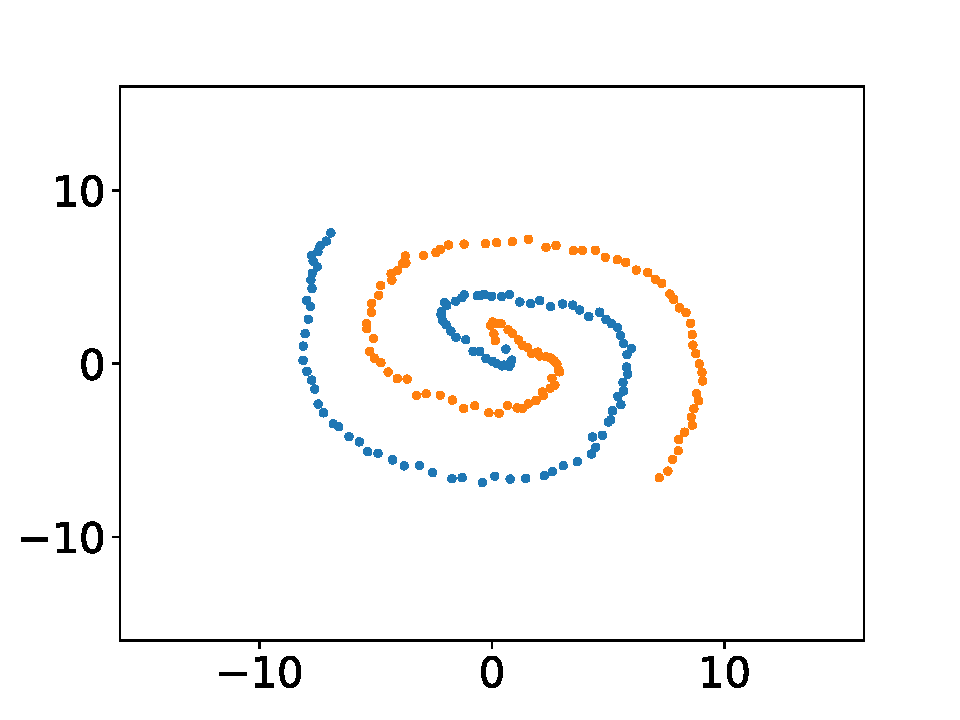
\includegraphics[scale=\imagescale]{figures/results/best_ckpt_2021_01_14_s_5_r_0.1_h_0.2_mu_0.01_reg_1e-06_step_0.2.pdf}}; 
			\node [right= of b1] (b2) {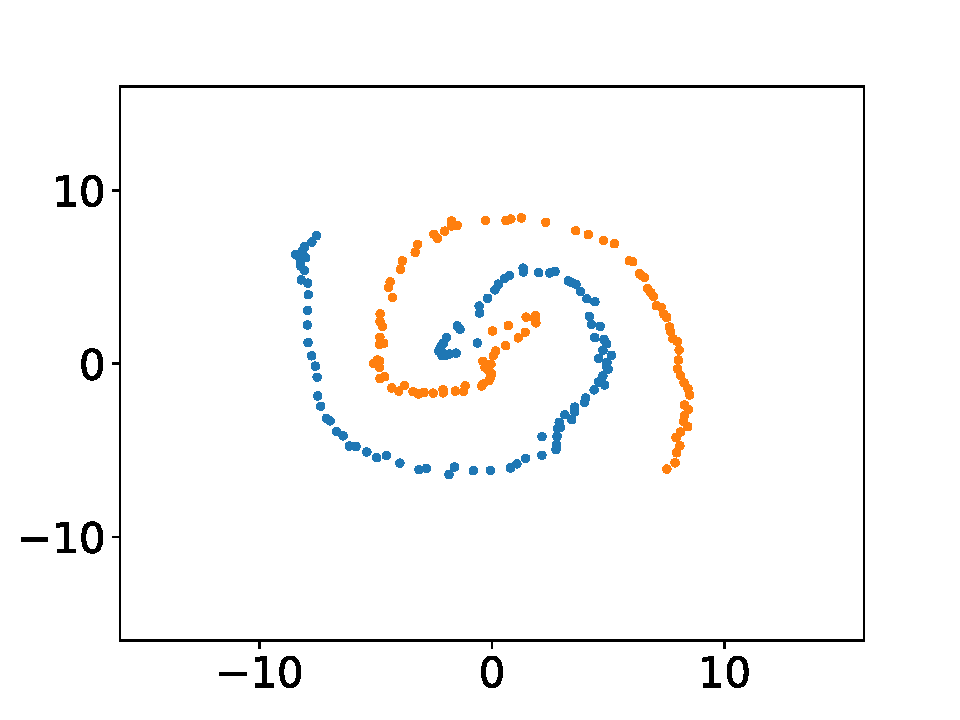
\includegraphics[scale=\imagescale]{figures/results/best_ckpt_2021_01_14_s_5_r_0.1_h_0.2_mu_0.01_reg_1e-06_step_0.4.pdf}};
			\node [right= of b2] (b3) {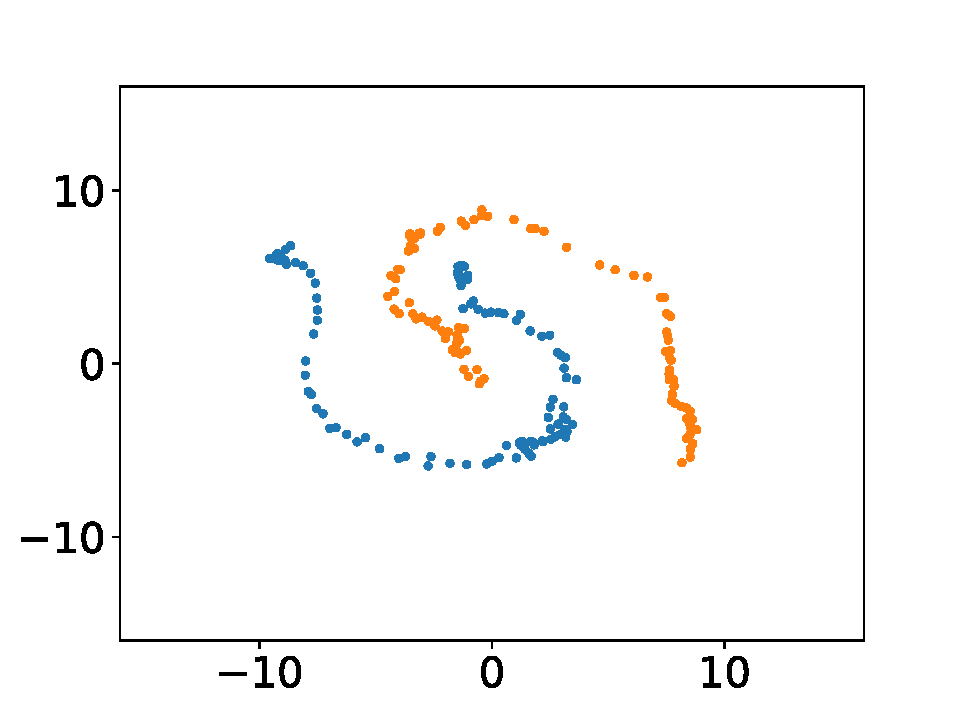
\includegraphics[scale=\imagescale]{figures/results/best_ckpt_2021_01_14_s_5_r_0.1_h_0.2_mu_0.01_reg_1e-06_step_0.6.pdf}};
			\node [right= of b3] (b4) {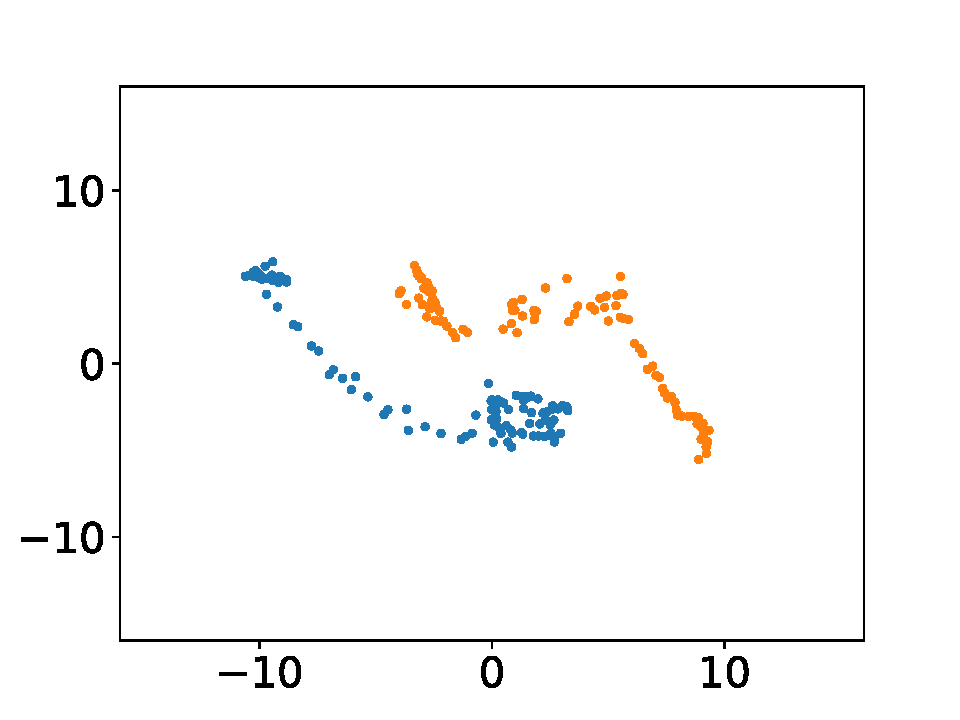
\includegraphics[scale=\imagescale]{figures/results/best_ckpt_2021_01_14_s_5_r_0.1_h_0.2_mu_0.01_reg_1e-06_step_0.8.pdf}};
			\node [right= of b4] (b5) {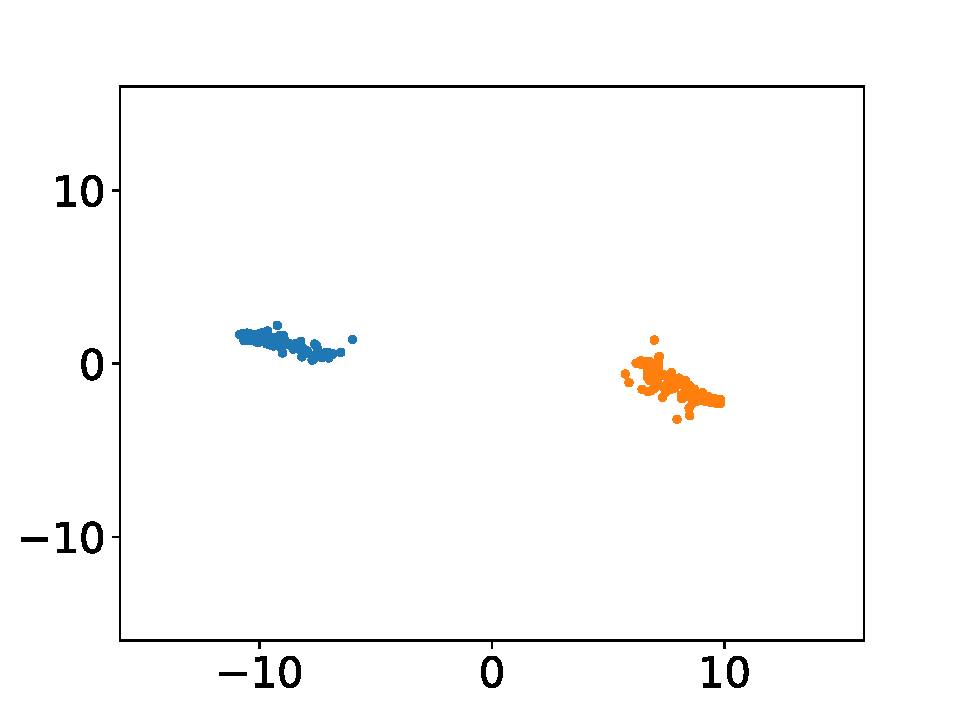
\includegraphics[scale=\imagescale]{figures/results/best_ckpt_2021_01_14_s_5_r_0.1_h_0.2_mu_0.01_reg_1e-06_step_1.0.pdf}};
			%
			\node [below= of b1] (c1) {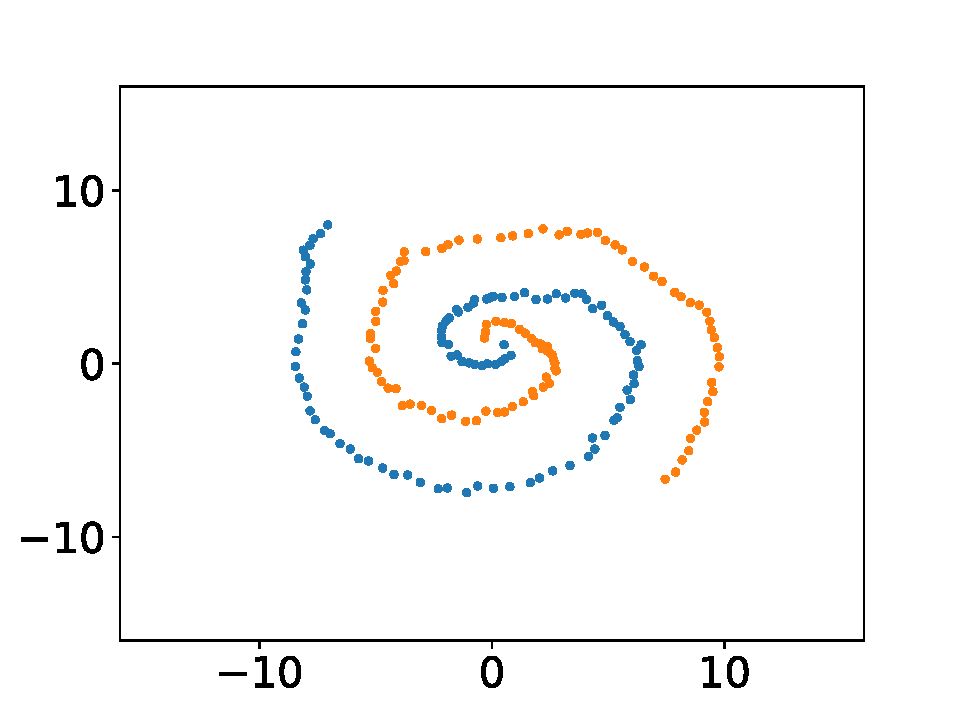
\includegraphics[scale=\imagescale]{figures/results/best_ckpt_2021_01_14_s_5_r_0.1_h_0.2_mu_0.02_reg_1e-06_step_0.2.pdf}}; 
			\node [right= of c1] (c2) {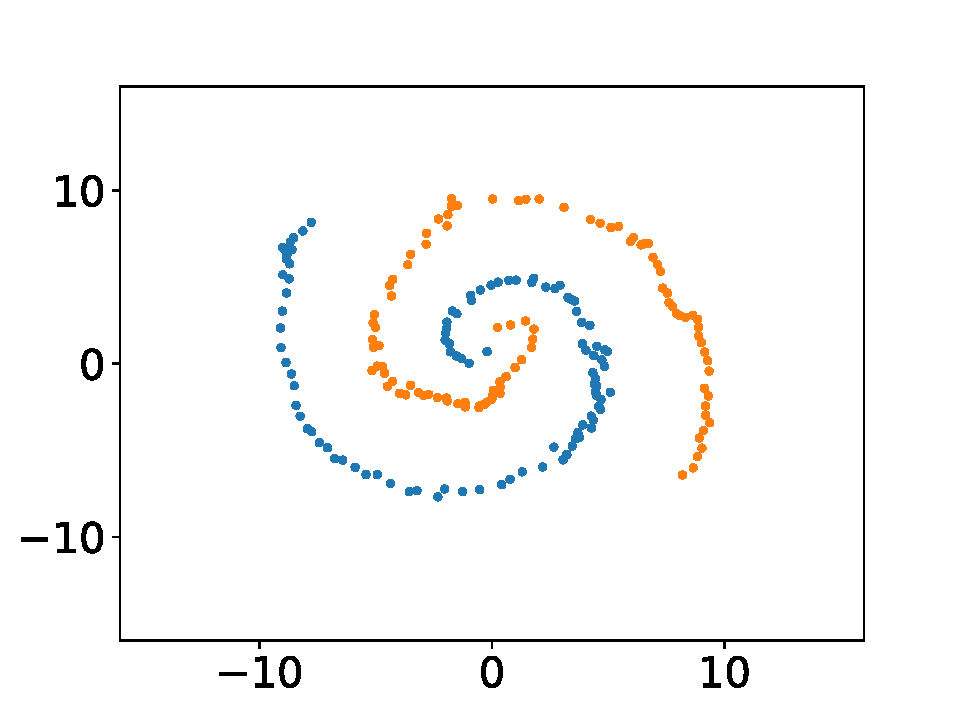
\includegraphics[scale=\imagescale]{figures/results/best_ckpt_2021_01_14_s_5_r_0.1_h_0.2_mu_0.02_reg_1e-06_step_0.4.pdf}};
			\node [right= of c2] (c3) {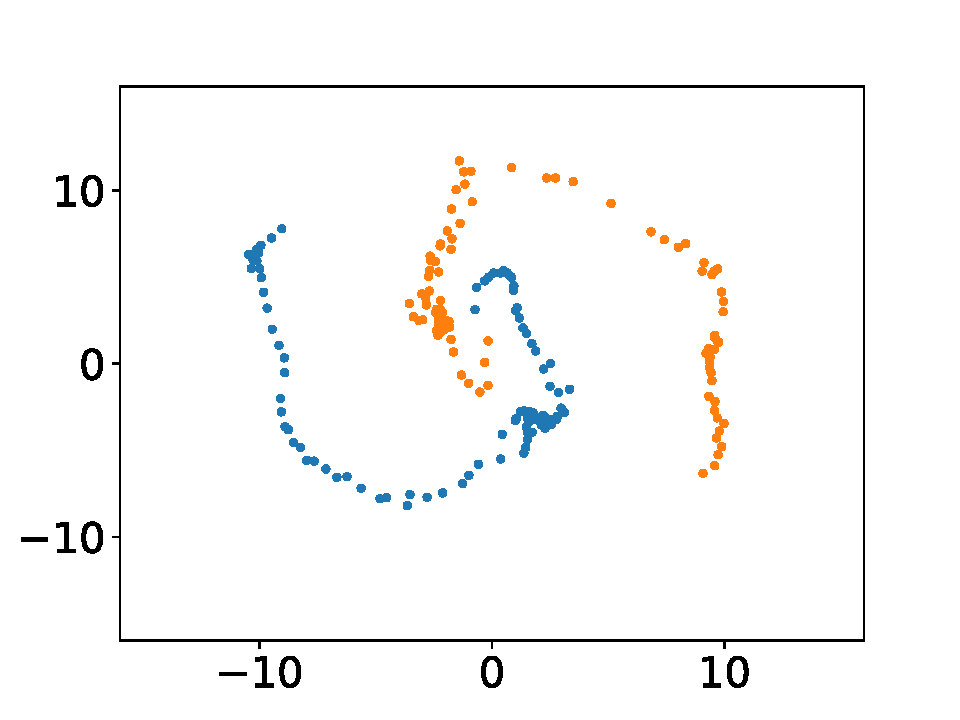
\includegraphics[scale=\imagescale]{figures/results/best_ckpt_2021_01_14_s_5_r_0.1_h_0.2_mu_0.02_reg_1e-06_step_0.6.pdf}};
			\node [right= of c3] (c4) {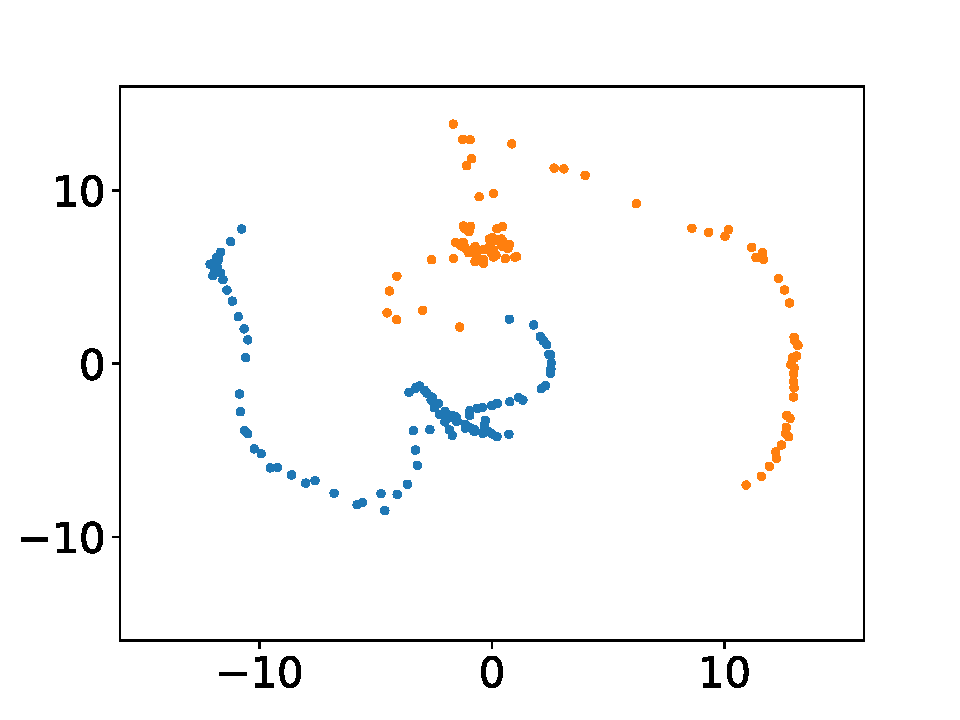
\includegraphics[scale=\imagescale]{figures/results/best_ckpt_2021_01_14_s_5_r_0.1_h_0.2_mu_0.02_reg_1e-06_step_0.8.pdf}};
			\node [right= of c4] (c5) {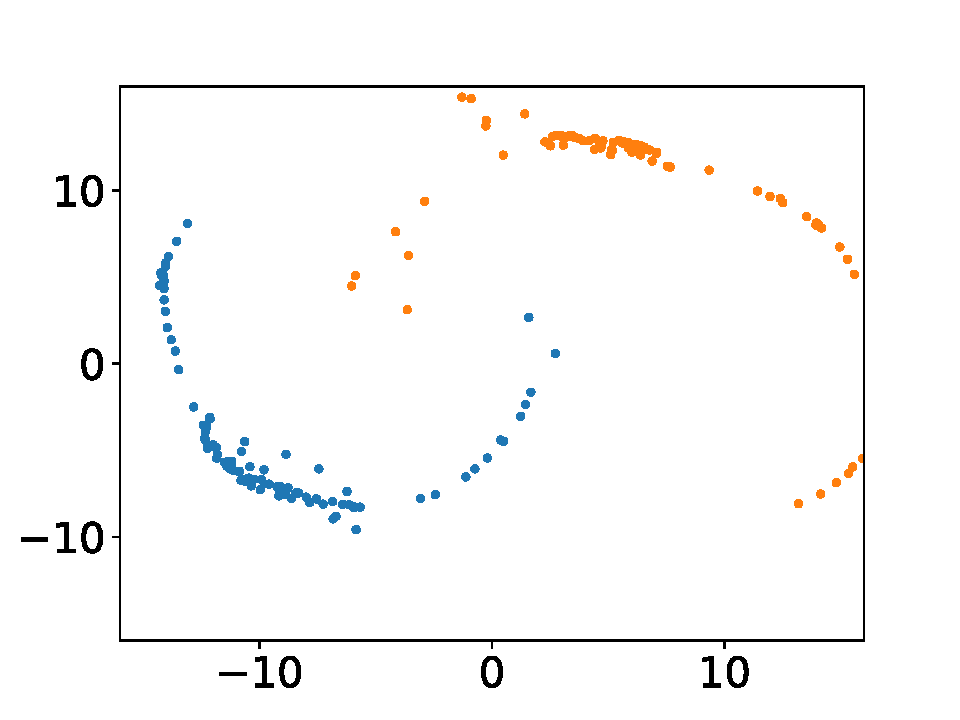
\includegraphics[scale=\imagescale]{figures/results/best_ckpt_2021_01_14_s_5_r_0.1_h_0.2_mu_0.02_reg_1e-06_step_1.0.pdf}};
			%
			\node [below= of c1] (d1) {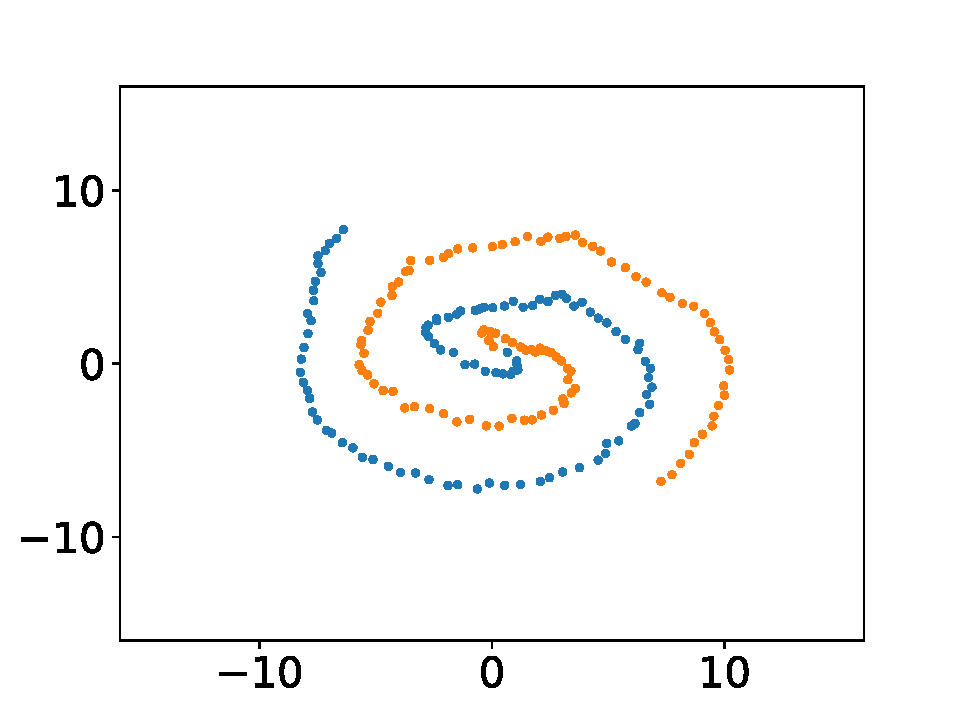
\includegraphics[scale=\imagescale]{figures/results/best_ckpt_2021_01_14_s_5_r_0.1_h_0.2_mu_0.03_reg_1e-06_step_0.2.pdf}}; 
			\node [right= of d1] (d2) {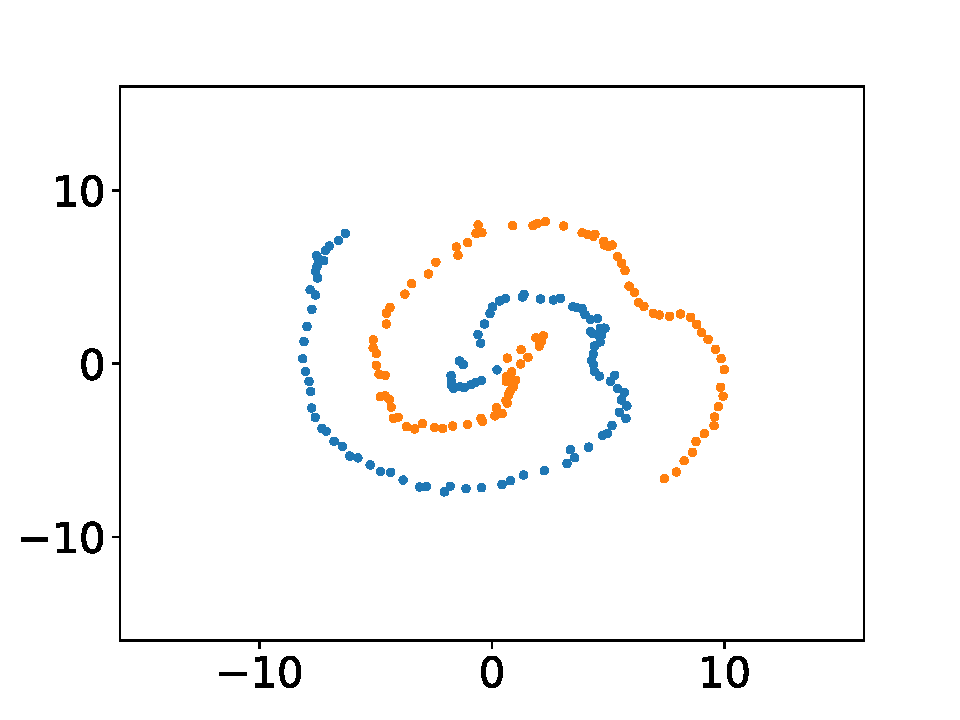
\includegraphics[scale=\imagescale]{figures/results/best_ckpt_2021_01_14_s_5_r_0.1_h_0.2_mu_0.03_reg_1e-06_step_0.4.pdf}};
			\node [right= of d2] (d3) {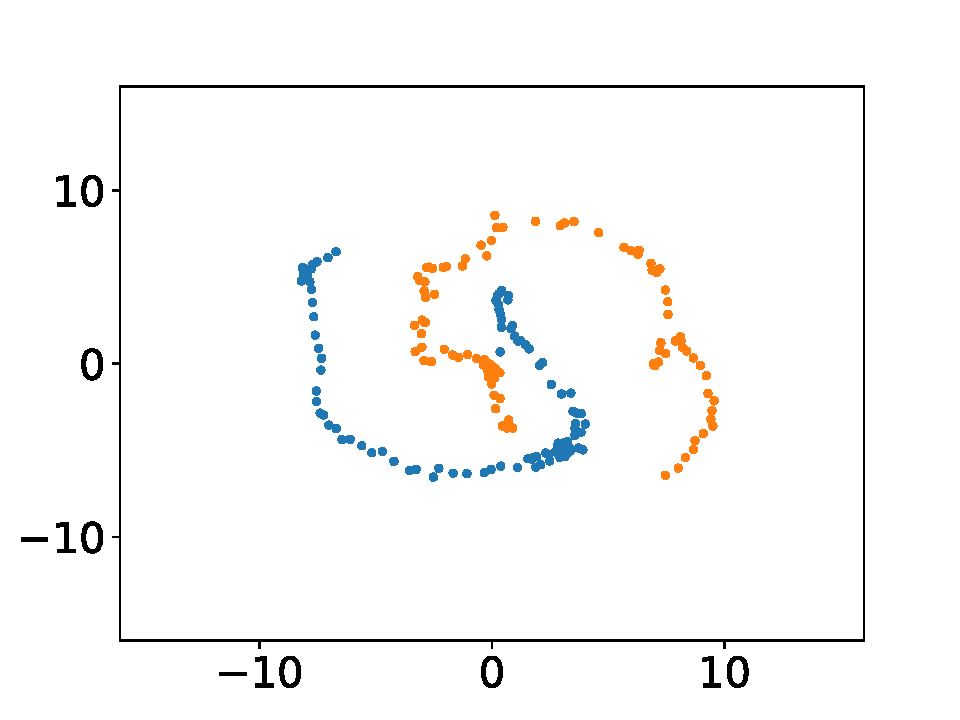
\includegraphics[scale=\imagescale]{figures/results/best_ckpt_2021_01_14_s_5_r_0.1_h_0.2_mu_0.03_reg_1e-06_step_0.6.pdf}};
			\node [right= of d3] (d4) {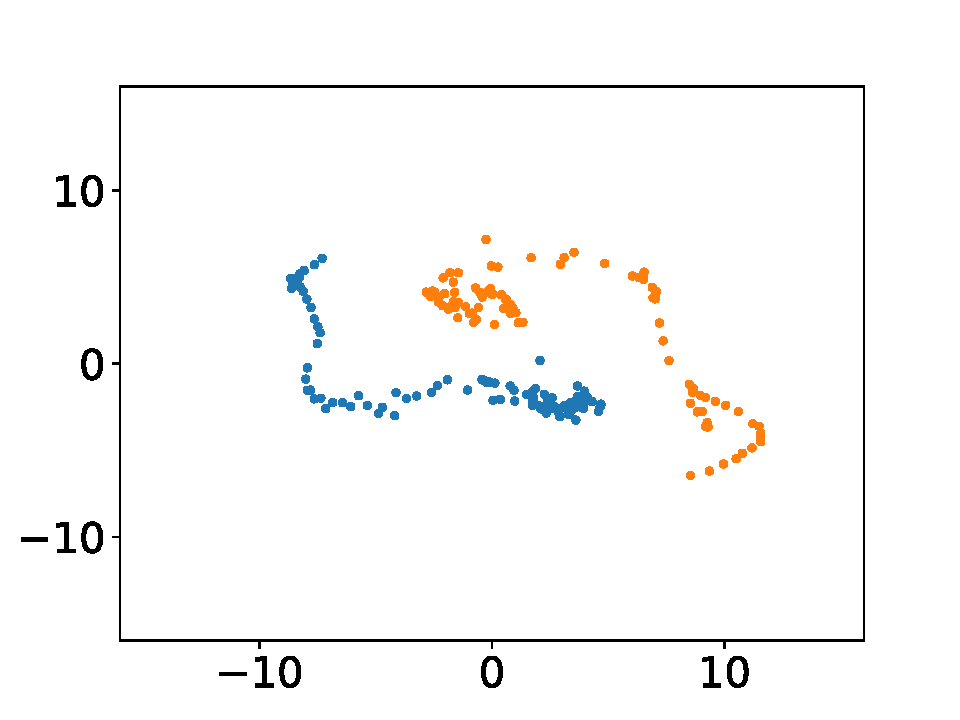
\includegraphics[scale=\imagescale]{figures/results/best_ckpt_2021_01_14_s_5_r_0.1_h_0.2_mu_0.03_reg_1e-06_step_0.8.pdf}};
			\node [right= of d4] (d5) {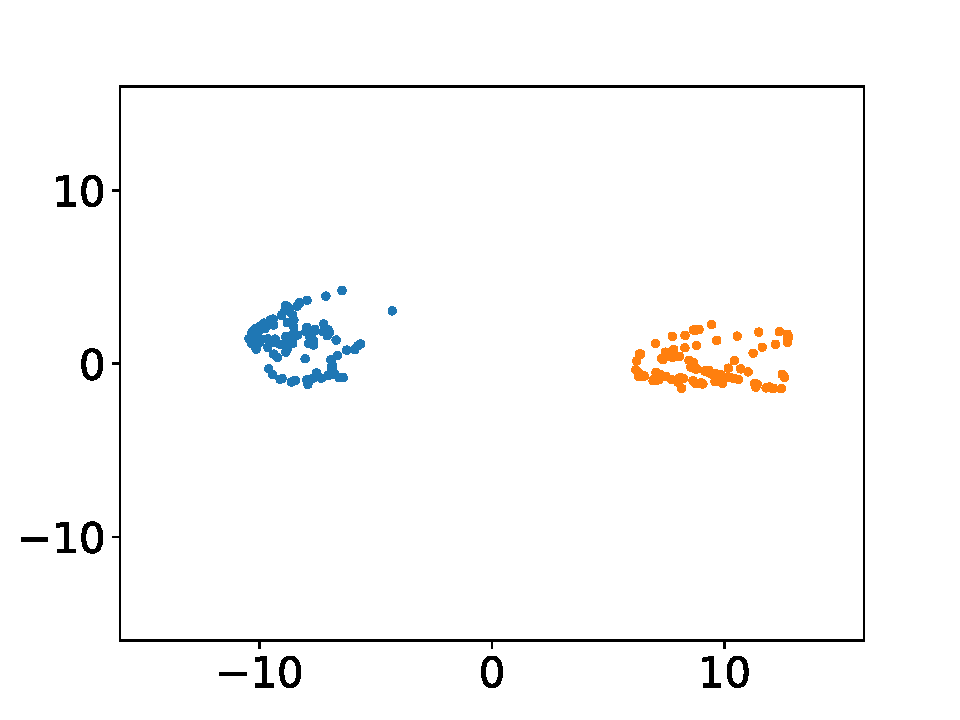
\includegraphics[scale=\imagescale]{figures/results/best_ckpt_2021_01_14_s_5_r_0.1_h_0.2_mu_0.03_reg_1e-06_step_1.0.pdf}};
			%
			\node [below= of d1] (e1) {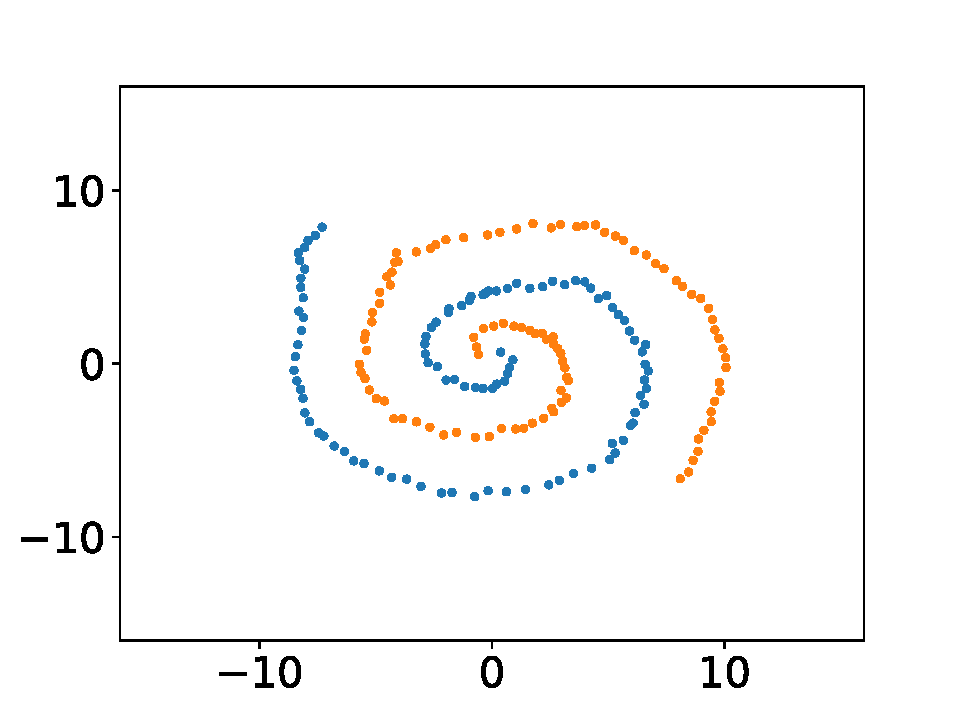
\includegraphics[scale=\imagescale]{figures/results/best_ckpt_2021_01_14_s_5_r_0.1_h_0.2_mu_0.05_reg_1e-06_step_0.2.pdf}}; 
			\node [right= of e1] (e2) {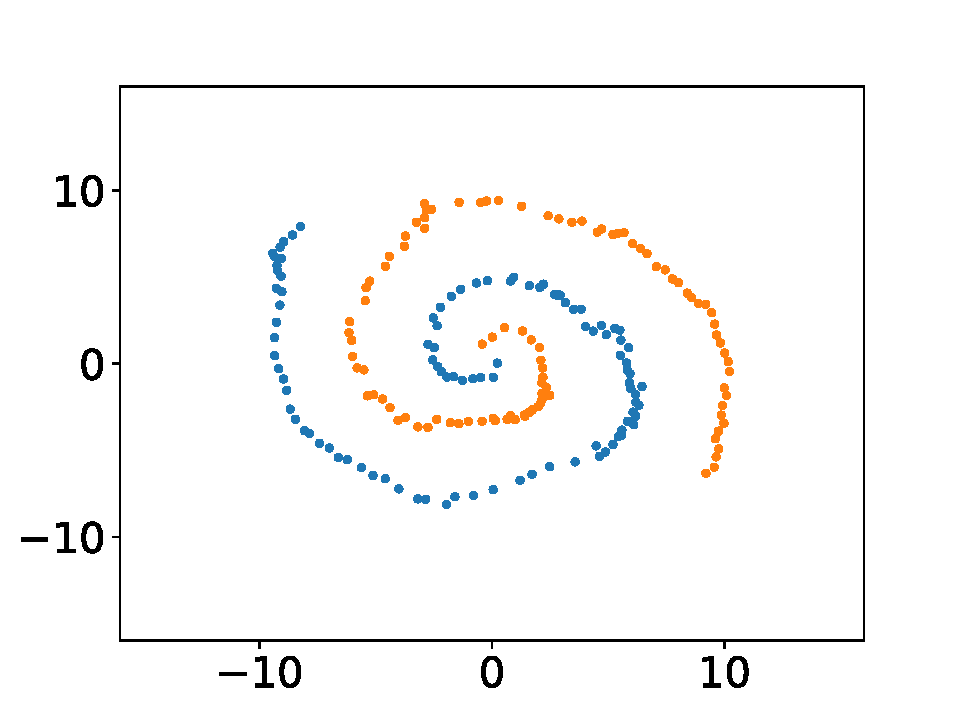
\includegraphics[scale=\imagescale]{figures/results/best_ckpt_2021_01_14_s_5_r_0.1_h_0.2_mu_0.05_reg_1e-06_step_0.4.pdf}};
			\node [right= of e2] (e3) {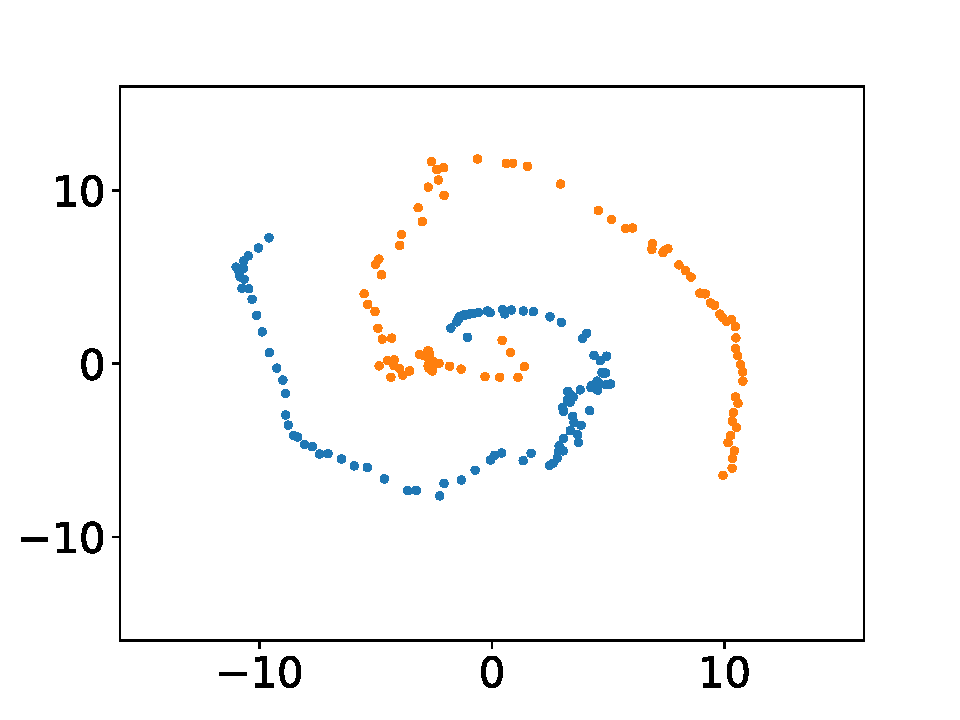
\includegraphics[scale=\imagescale]{figures/results/best_ckpt_2021_01_14_s_5_r_0.1_h_0.2_mu_0.05_reg_1e-06_step_0.6.pdf}};
			\node [right= of e3] (e4) {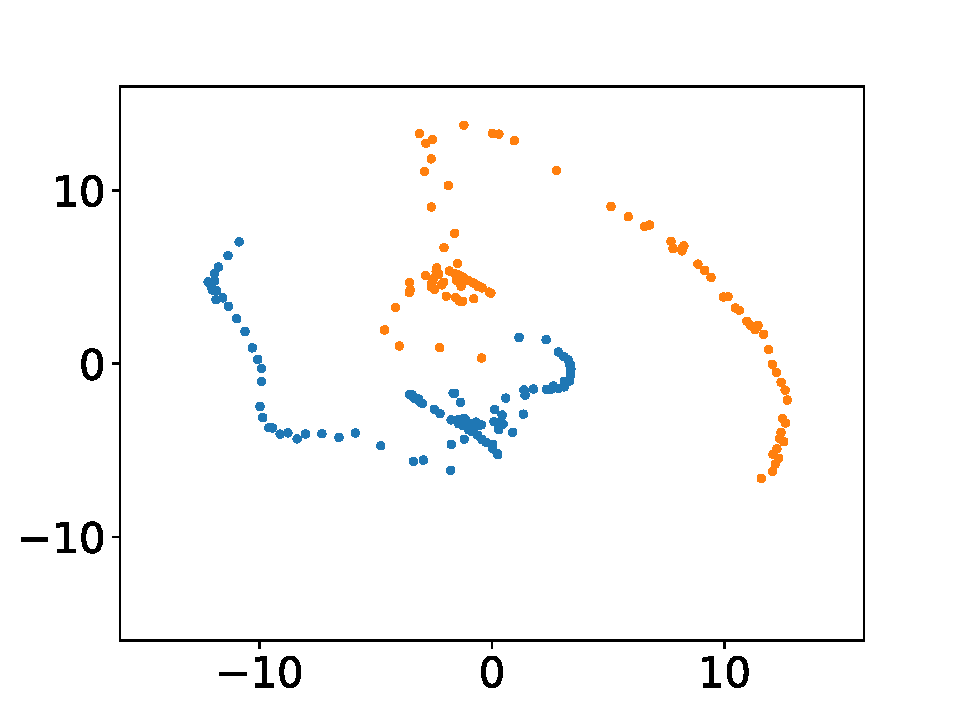
\includegraphics[scale=\imagescale]{figures/results/best_ckpt_2021_01_14_s_5_r_0.1_h_0.2_mu_0.05_reg_1e-06_step_0.8.pdf}};
			\node [right= of e4] (e5) {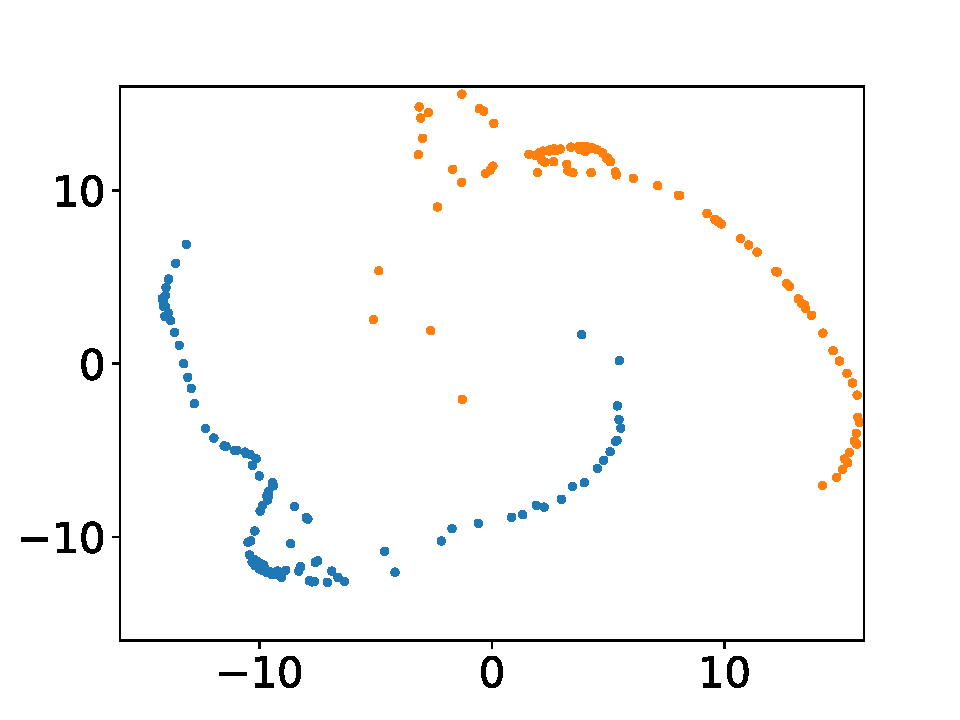
\includegraphics[scale=\imagescale]{figures/results/best_ckpt_2021_01_14_s_5_r_0.1_h_0.2_mu_0.05_reg_1e-06_step_1.0.pdf}};
			%
			\node [below= of e1] (a1) {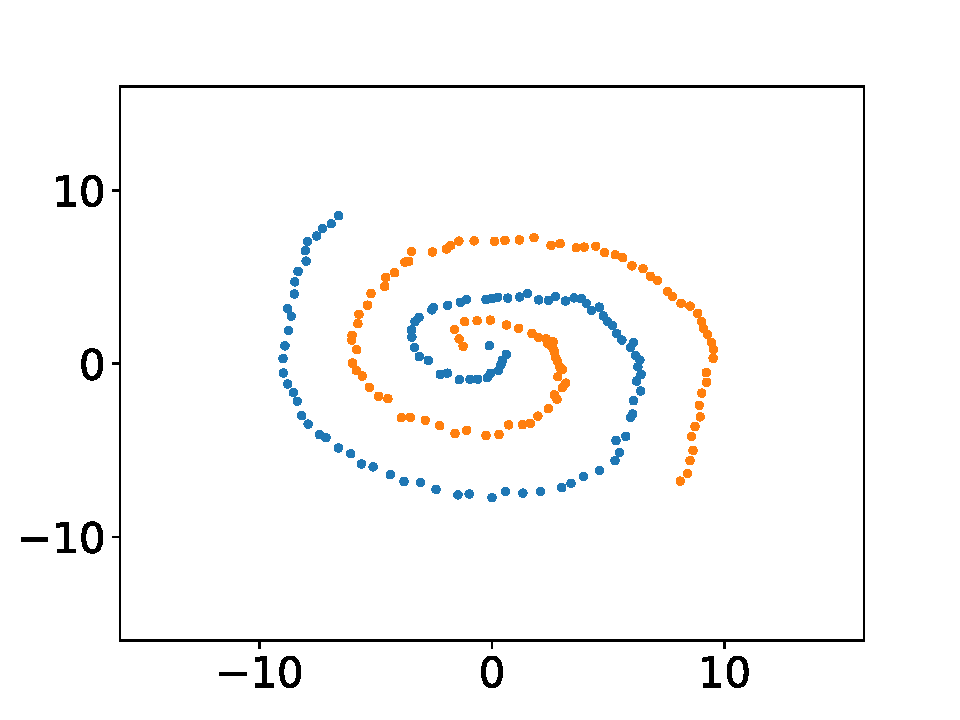
\includegraphics[scale=\imagescale]{figures/results/best_ckpt_2021_01_14_s_5_r_0.1_h_0.2_mu_0.1_reg_1e-06_step_0.2.pdf}}; 
			\node [right= of a1] (a2) {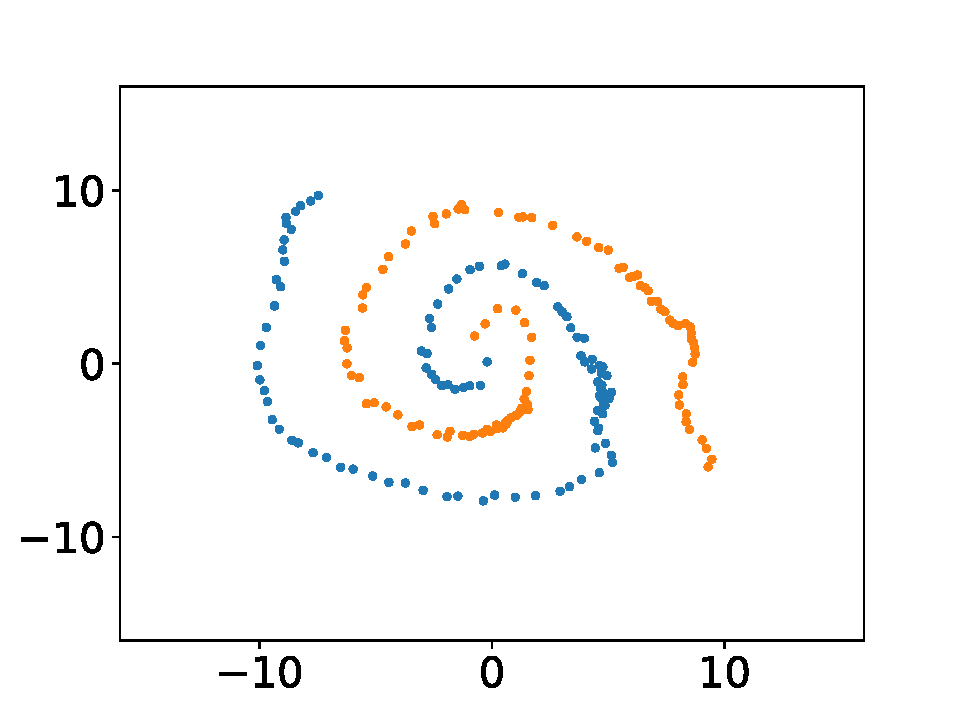
\includegraphics[scale=\imagescale]{figures/results/best_ckpt_2021_01_14_s_5_r_0.1_h_0.2_mu_0.1_reg_1e-06_step_0.4.pdf}};
			\node [right= of a2] (a3) {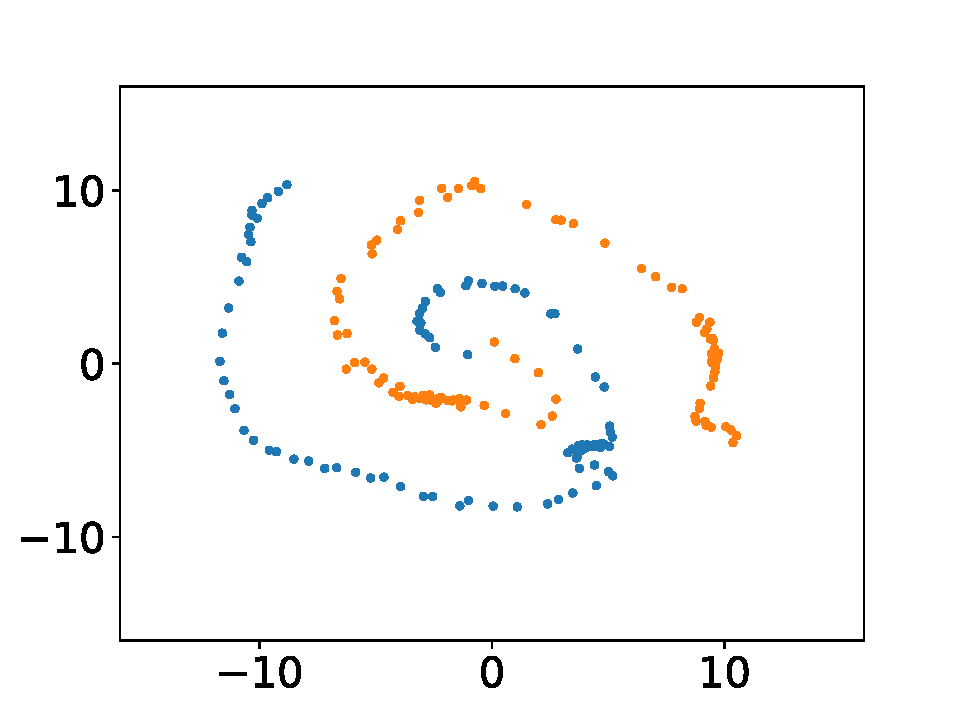
\includegraphics[scale=\imagescale]{figures/results/best_ckpt_2021_01_14_s_5_r_0.1_h_0.2_mu_0.1_reg_1e-06_step_0.6.pdf}};
			\node [right= of a3] (a4) {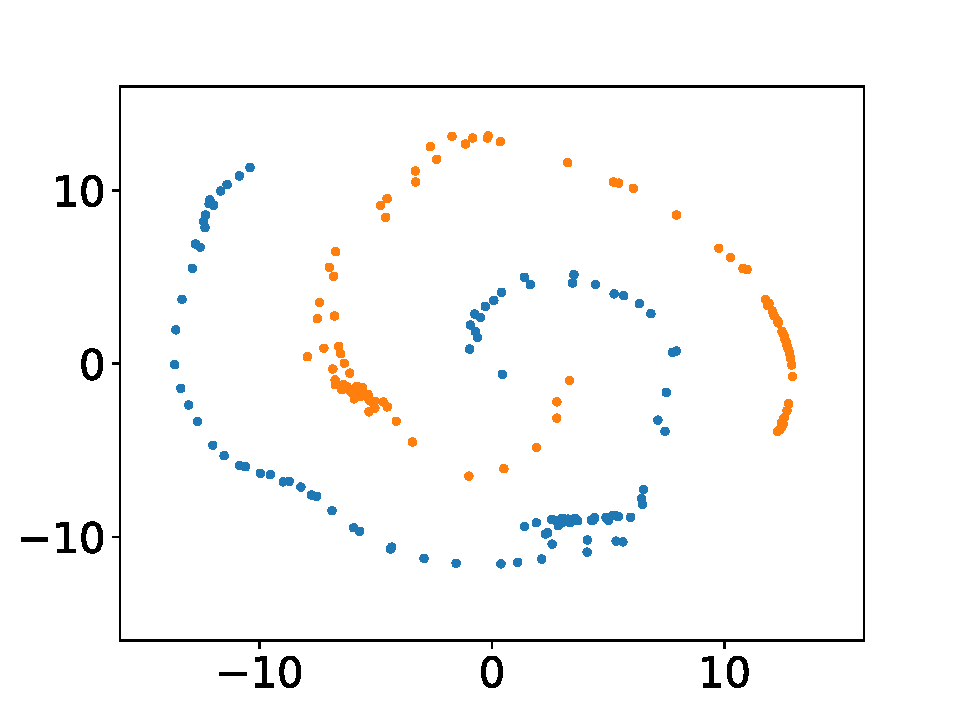
\includegraphics[scale=\imagescale]{figures/results/best_ckpt_2021_01_14_s_5_r_0.1_h_0.2_mu_0.1_reg_1e-06_step_0.8.pdf}};
			\node [right= of a4] (a5) {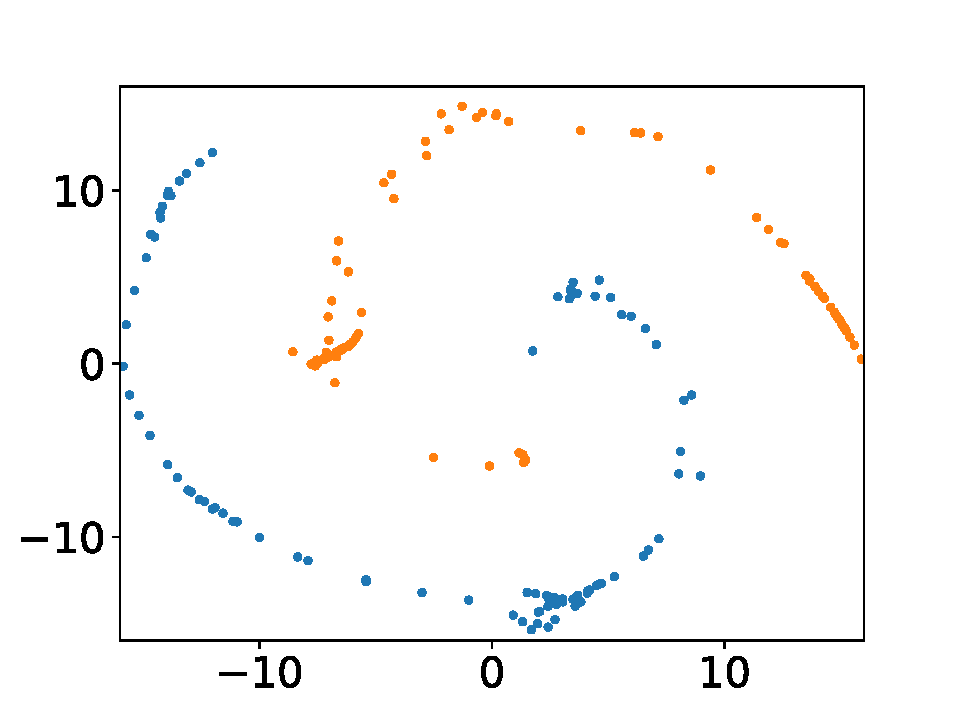
\includegraphics[scale=\imagescale]{figures/results/best_ckpt_2021_01_14_s_5_r_0.1_h_0.2_mu_0.1_reg_1e-06_step_1.0.pdf}};
			%
			\node [below= of a1] (f1) {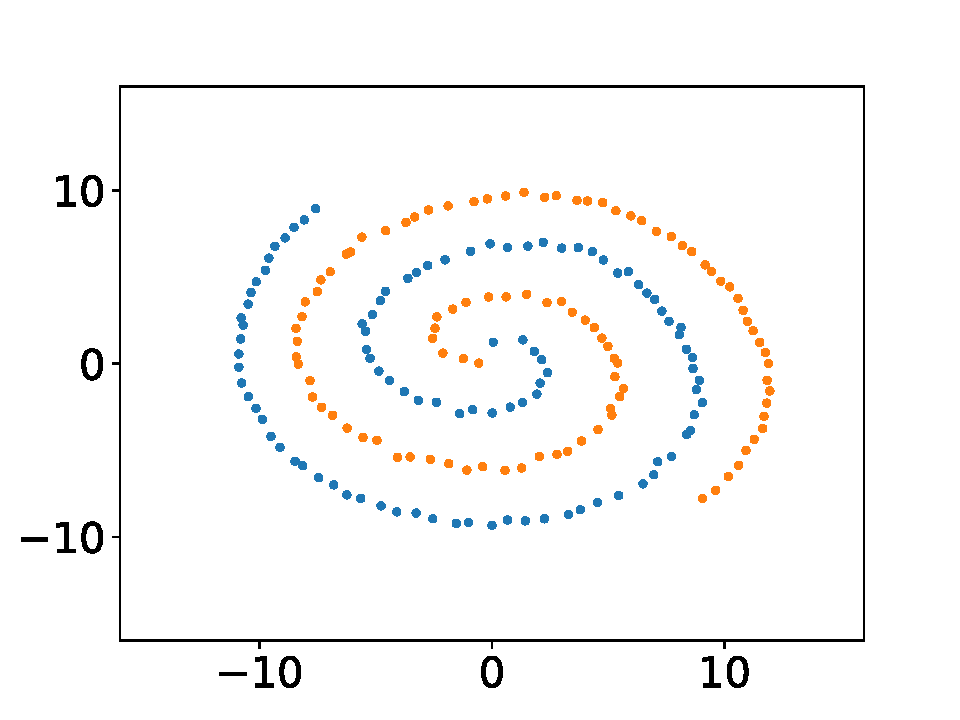
\includegraphics[scale=\imagescale]{figures/results/best_ckpt_2021_02_16_s_5_r_0.1_h_0.2_mu_0.5_reg_1e-06_step_0.2.pdf}}; 
			\node [right= of f1] (f2) {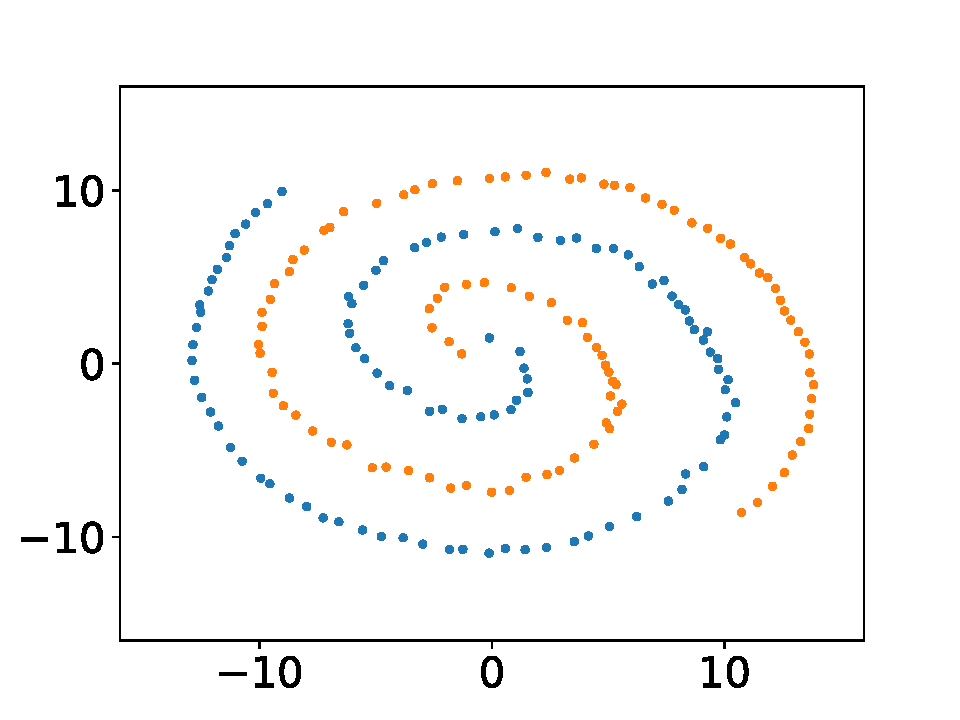
\includegraphics[scale=\imagescale]{figures/results/best_ckpt_2021_02_16_s_5_r_0.1_h_0.2_mu_0.5_reg_1e-06_step_0.4.pdf}};
			\node [right= of f2] (f3) {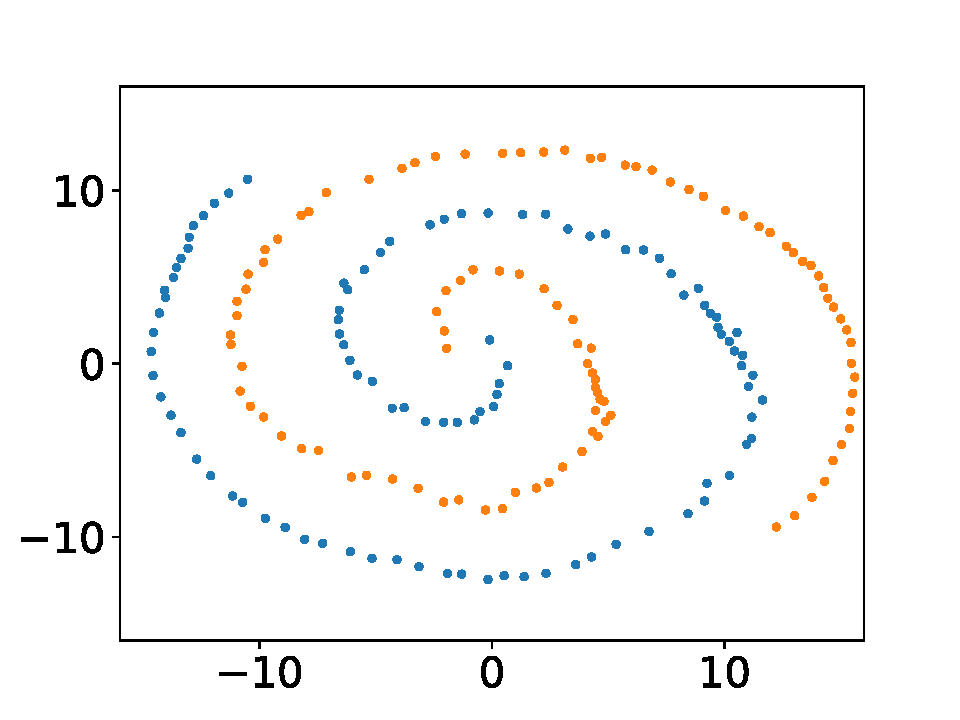
\includegraphics[scale=\imagescale]{figures/results/best_ckpt_2021_02_16_s_5_r_0.1_h_0.2_mu_0.5_reg_1e-06_step_0.6.pdf}};
			\node [right= of f3] (f4) {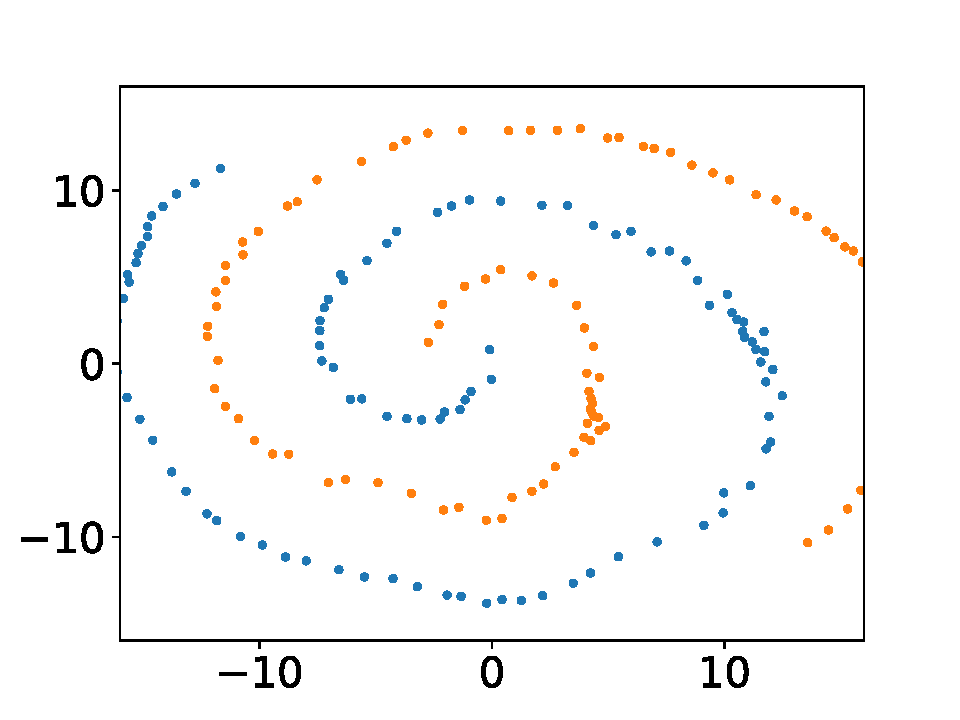
\includegraphics[scale=\imagescale]{figures/results/best_ckpt_2021_02_16_s_5_r_0.1_h_0.2_mu_0.5_reg_1e-06_step_0.8.pdf}};
			\node [right= of f4] (f5) {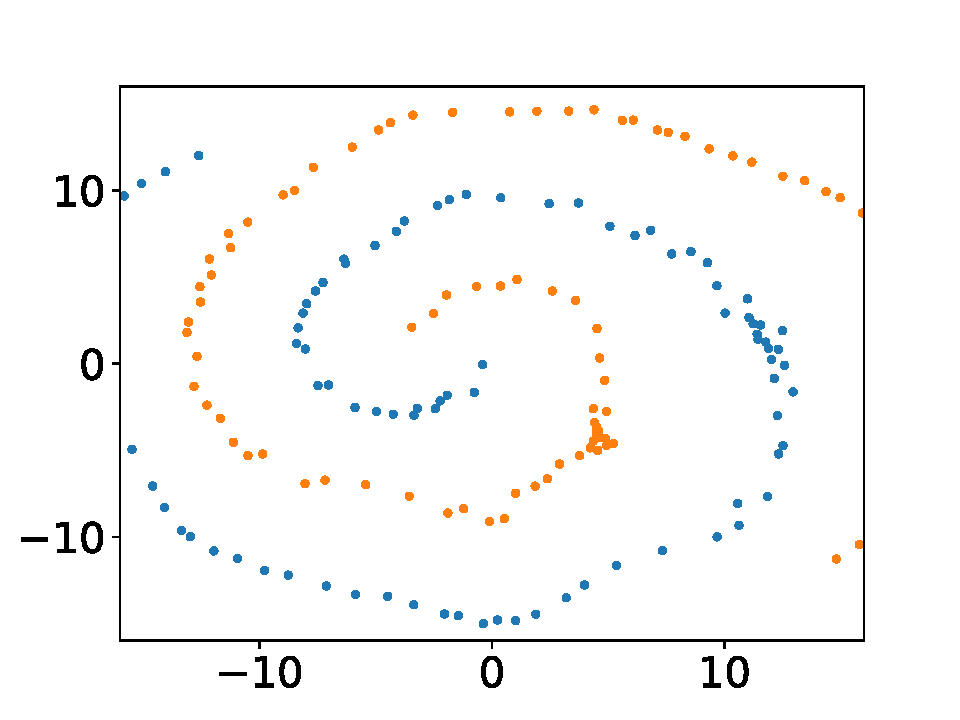
\includegraphics[scale=\imagescale]{figures/results/best_ckpt_2021_02_16_s_5_r_0.1_h_0.2_mu_0.5_reg_1e-06_step_1.0.pdf}};
			%
			\node[left= -0.35cm of a1] (a0) {$\mu=0.1$};
			\node[left= -0.35cm of b1] (b0) {$\mu=0.01$};
			\node[left= -0.35cm of c1] (c0) {$\mu=0.02$};
			\node[left= -0.35cm of d1] (d0) {$\mu=0.03$};
			\node[left= -0.35cm of e1] (e0) {$\mu=0.05$};
			\node[left= -0.35cm of f1] (f0) {$\mu=0.5$};
			%
			\node[above= -0.1cm of b1] (z1) {$t=0.2$};
			\node[above= -0.1cm of b2] (z2) {$t=0.4$};
			\node[above= -0.1cm of b3] (z3) {$t=0.6$};
			\node[above= -0.1cm of b4] (z4) {$t=0.8$};
			\node[above= -0.1cm of b5] (z5) {$t=1.0$};
		\end{tikzpicture}
	}
	\caption{Here will be the results of the experiments.}
	\label{fig:results-swiss-roll}
\end{figure}

\cref{fig:results-swiss-roll} shows experimental results for step 3 of the algorithm.
Each plot represents the locations $q(t)$ at a point in time $t \in \{0.2, 0.4, 0.6, 0.8, 1\}$ for different parameters $\mu$.
Because of $q(0) = X$, at time $t = 0$ the points are still at their original positions (\cref{fig:dataset}).
The magnitude of the points' movement (or rather the deformation of the space) depends on the balancing parameter $\mu$.
As $\mu$ increases, the deformation of the space is penalized to a stronger degree.
This is due to the fact that the norm of $v_k$ in \cref{prob:min-v-f} decreases the more similar $v_k$ is to the zero function.
Hence, weighting the norms of $v_k$ more compared to the loss $l$ results in less space deformation.
This can be seen in the rightmost column ($t=1$):
The point clouds stay closer to their original positions as $\mu$ increases.

The plot at $(\mu=0.03, t=1)$ is of great interest, as it is not in line with the other plots, which at $t=1$ mostly show monotonously decreasing space deformation when $\mu$ increases.
From $\mu = 0.02$ to $\mu = 0.03$, this trend is inverted.
It is not clear what exactly causes this phenomenon.
One explanation would that the optimizer performed poorly for $\mu=0.02$ and the space was transformed to a lesser degree than it should have for the optimal momentum.
However, this has been ruled out by repeated experiments with $\mu = 0.02$.
This leads to another possible explanation, which is that the optimization algorithm (here, a version of gradient descent) is not performing well.
If the optimizer struggles to approximate the optimal initial momentum $p(0)$ and mostly remains at sub-optimal points or local minima, it could still -- by chance -- hit better points.
This interpretation would imply that in all other experiments, the optimum could not be approximated properly.
Finally, numerical imprecisions in general could be the source for the outlier.
They could arise at several steps in the algorithm, e.g. the integration scheme or the matrix inversion.

Overall, the experimental results come close to those presented by \citet{owhadi20}, although the deformations, here, are stronger.
For $\mu = 0.01$, for example, the spirals are still visible in \cite{owhadi20} whereas in this work, the points form linearly separable clouds.
Only at $\mu = 0.05$ does the deformation approximately match that in \cite{owhadi20}.
The cause of these differences remain unclear.
A possible explanation would be the Tikhonov regularization that was applied here.
It could also be possible that the search for the optimal momentum was performed for more iterations or that different optimization algorithms were used.

The experiments visualize \citet{owhadi20}'s interpretation of mechanical regression as idea registration, which he compares to image registration.
In mechanical regression, it is not the images or landmarks that are transformed, but general data points.
The two-dimensional example shows the overlap between these notions.
The data points are still transformed, but their "targets" cannot be seen -- they are intrinsic to the algorithm.

\subsubsection{Remarks on the Implementation}

The pseudocode in \cref{fig:algo} can be implemented fairly straight forward.
However, there are some tricks that make it easier, some of which are presented here.

The first simplification lies in the implementation of the inner product on $\cX = \R^2$, which is just the standard scalar product.
In order to fully make use of modern tensor-processing frameworks' parallel processing abilities, expressing the scalar product of $\cX^N$ (which is defined as $\sum_{i=1}^N \left<x_{1, i}, x_{2, i}\right>_\cX$ for $x_1, x_2 \in \cX^N$) in terms of matrix operations is highly desirable.
\cref{cor:matrix-ring-equivalence} provides an option to do so.
We simply (bijectivly) map vectors from $\cX^N$ to $\R^{2N}$.
Then we can perform standard vector-vector multiplication efficiently using the framework's capabilities and, if required, map the result back to $\cX^N$.
The application of a block operator matrix to a vector can be performed similarly, employing \cref{cor:matrix-vector-equivalence}:
Block operator matrices are mapped from $L(\cX^N, \cX^N)$ to $\R^{2N \times 2N}$ and subsequently standard matrix-vector multiplication can be carried out.
It turned out that it is easier to work in the spaces $\R^{2N}$ and $\R^{2N \times 2N}$ by default and switch to the isomorphic ones only when necessary.

Another potentially difficult step to implement is the gradient of $\fH$ with respect to $q$, especially in cases like \cref{eq:leapfrog-p.5,eq:leapfrog-p1} where no closed form formula is available.
A solution for this would be to approximate the gradient using two-point methods such as the left/right sided or symmetric difference quotient.
However, some modern programming languages or frameworks therein (like the Julia language or Tensorflow and PyTorch for Python) provide automatic differentiating capabilities.
Those are not only simpler to implement but also computationally more efficient, which strongly encourages their use.

As the experiments showed, using the optimal recovery loss in its pure form does not seem to be possible (at least for the Swiss Roll dataset).
Recall \cref{eq:optimal-recovery-loss-closed-form} where we identified the loss as $l(X, Y) = Y^\T \mathbf{K}(X, X)^{-1} Y$.
Note that it involves computing $\mathbf{K}(X, X)^{-1}$, or rather solving the linear system $\mathbf{K}(X, X)^{-1} Y$.
That system, involving a $(200\times200)$ matrix, proved to be ill-conditioned, which gave rise to some numerical issues and compromised the minimization process.
Hence, some matrix regularization was applied:
Adding a small perturbation $\lambda$ to the diagonal elements (in the experiments $\lambda = 10^{-6}$ was used) alleviated this problem.
This method is also known as Tikhonov regularization.
However, this effectively changed the loss to the ridge regression loss employing the empirical squared error, which reads (\cref{eq:ridge-regression-loss-se-closed-form}):
\begin{equation}
	l(X, Y) = \lambda Y^\T (\mathbf{K}(X, X) + \lambda \mathbbm{1}_N)^{-1} Y \ ,
\end{equation}
the only difference being the initial scaling by $\lambda$.

The Python implementation used in the experiments is available at \url{https://github.com/NKlug/thesis-mechanical-regression}.
The use of Google's Tensorflow framework \cite{tensorflow15} made it particularly easy to leverage GPU acceleration, automated gradients and pre-implemented optimization algorithms.
